
\begin{table}
\caption{EMBERS system statistics}
 \centering
 \begin{tabular}{|l|l|l|l|l|}
 \hline
 Archived data     & 12.4 TB                  \\ \hline
 Archive size & ca. 3 billion messages   \\ \hline
 Data throughput   & 200-2000 messages/sec  \\ \hline
 Daily ingest & 15 GB \\ \hline
 System memory & 50 GB \\ \hline
 System core & 16 vCPUs \\ \hline
 System output & ca. 40 warnings/day \\ \hline
\end{tabular}
\label{tab:stats}
\end{table}



\section{Linguistic Preprocessing}

All textual input (e.g., tweets, news articles, blog postings) is
subjected to shallow linguistic processing prior to analysis.  This
involves identifying the language of the document, distinguishing the
the words (tokenization), normalizing words for inflection
(lemmatization), and identifying expressions referring to people,
places, dates and other entities and classifying them (named entity extraction). As our
data set is multilingual, with Spanish, Portuguese and English
predominating, we use a suite of multilingual commercial tools for
this processing.\footnote{BASIS Technology's Rossette Linguistic Platform}

This linguistic preprocessing serves as input to subsequent deeper semantic analysis in which 
date expressions are normalized and deindexed, the geographic focus of the text identified.
This processing chain is illustrated in Fig.~\ref{fig:enrichment}.

\begin{figure}
    \centering
    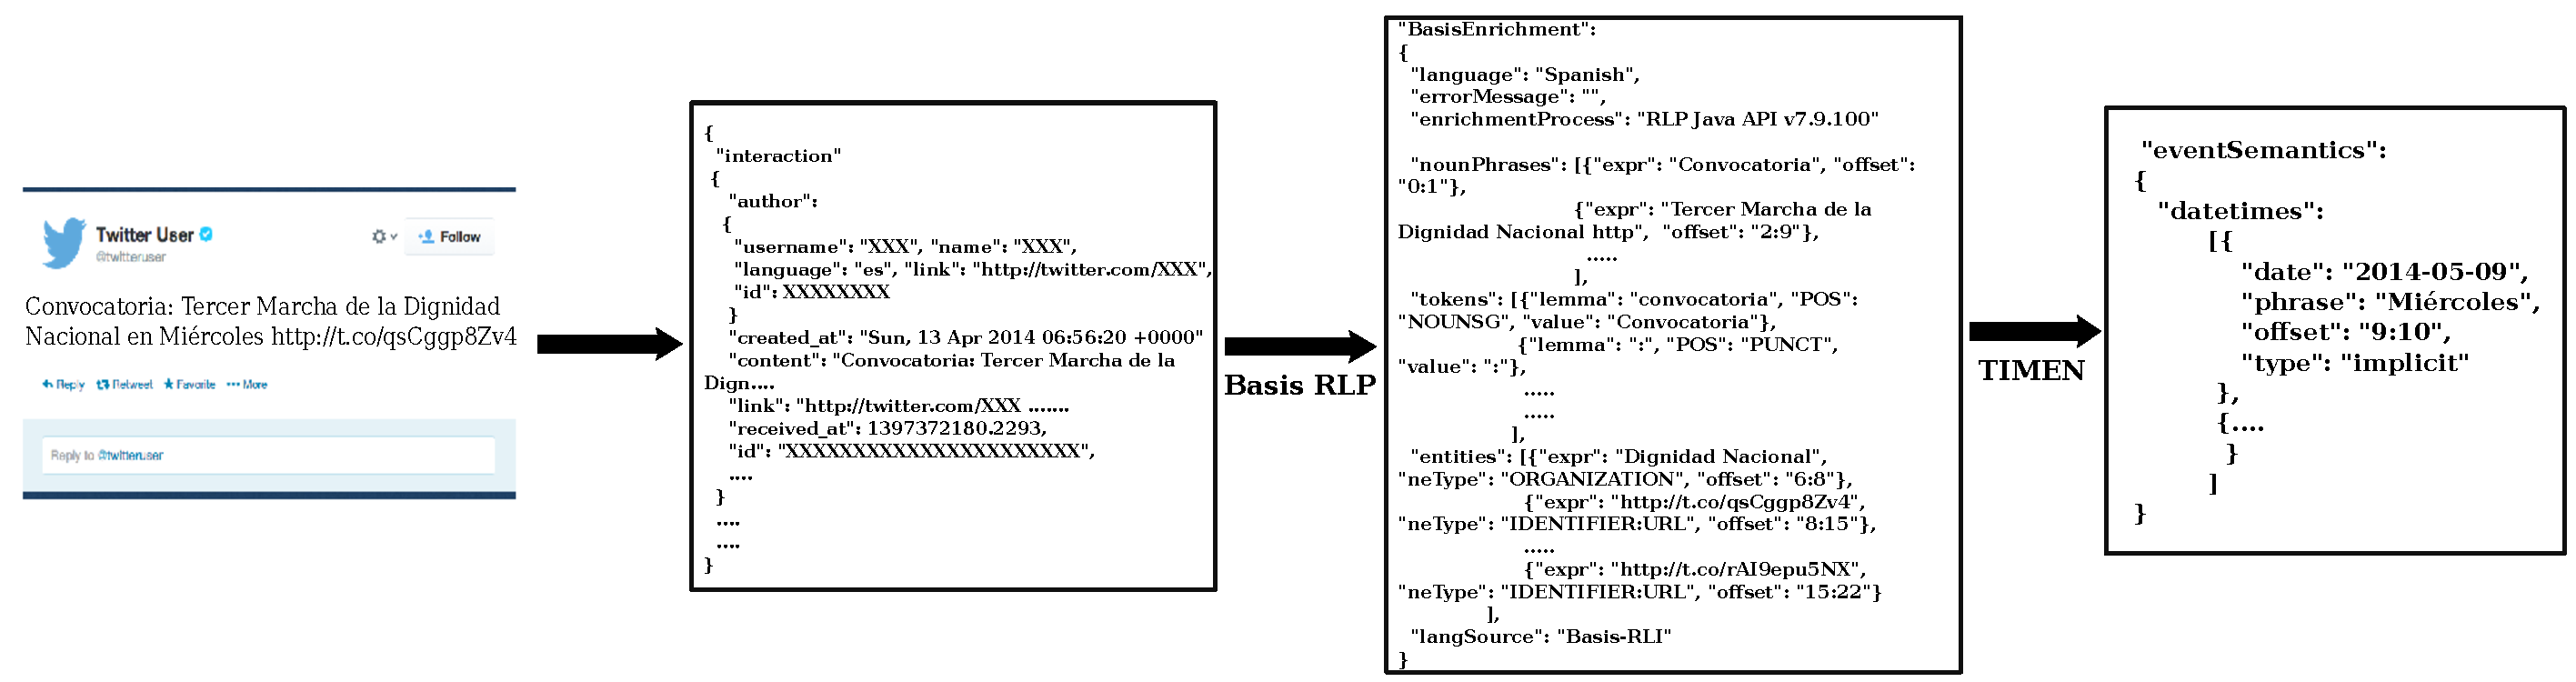
\includegraphics[width=0.5\textwidth]{enrichment}
    \caption{Message Enrichment}
    \label{fig:enrichment}
\end{figure}

Date processing is particularly crucial to the identification of
future oriented statements. We use the TIMEN \cite{LlorensDGS12} date
normalization package to normalize and deindex expressions referring
to days in English, Spanish and Portuguese.  This system makes use of
meta-data, such as the day of publication, and other information about
the linguistic context of the date expression to determine for each date expression,
what day (or week, month or year) it refers to.  For example in a tweet produced on June 10, 2014, the occurrence of 
the term {\em Friday} used in a future-tense sentence {\em We'll get together on Friday} will be interpreted as July 13, 2014.
Each expression identified as a date by the RLP preprocessor is normalized in this way.


\section{Geo-Coding}
\label{subsection:geocoding}

After preprocessing, documents are geocoded with a specification of the geographical focus of the text---specified as a city, state, country tripple.
We make use of different geocoding methodologies for geo-coding news/blogs and for geo-coding Twitter postings.




\subsection{Twitter}

For tweets, the geo-focus of the message is generated by a fairly
simple set of heuristics.  In particular, Twitter
geocoding is achieved by first considering the most reliable but least
available source, the geotag of the tweet itself (this is available
for about 10% of our sample from Twitter). This provide an exact
geographic locations that can be reverse geocoded into a place names
and this used as the geo-focus. We find the nearest geo-coded point in
our extended gazetteer (using the KD-Tree algorithm) for this
purpose. If the tweet is not geocoded, we consider Twitter ``places''
metadata and use place names present in these metadata fields to
geocode the place names into geographical coordinates.  Finally, if
none of this is available, we consider the text fields contained in
the user profile (location, description) as well as the tweet text
itself to find mentions of relevant locations.  Additional toponym disambiguiation heuristics are used to
identify the actual referent of the mention.

\subsection{Facebook}
Similar methods are used to geocode event data extracted from Facebook Events pages.   Since only Facebook Events that have a venue are used and a venue of a Facebook Event generally contains a latitude, longitude, and physical address information identifying the locatino is a fairly trivial task.  In cases where only latitude and longitude are given we apply reverse-geocoding mechanisms similar to those used for Twitter.


\subsection{News/Blogs}

For longer articles such as news articles, the geo-focus of the message is identified using much more complex methods
To extract the protest location from news articles, we use \emph{probabilistic soft logic} (PSL) described in ~\ref{section:PSL} to build a model that performs robust, probabilistic inference given noisy signals. PSL takes a set of weighted, logic-like rules and converts them into a continuous probability distribution over the unknown truth values of logical facts. These truth values in PSL are relaxed into the $[0,1]$ interval. We use this mechanism to build a model that infers the semantic location of an article by weighing evidence coming from the Basis entity extractions and information in the World Gazatteer. 

The primary rules in the model encode the effect that Basis-extracted location strings that match to gazatteer aliases are indicators of the article's location, whether they be country, state, or city aliases. Each of these implications is conjuncted with an prior for ambiguous, overloaded aliases that is proportional to the population of the gazetteer location. For example, if the string ``Los Angeles'' appears in the article, it could refer to either Los Angeles, California, or Los \'{A}ngeles in Argentina or Chile. Given no other information, our model would infer a higher truth value for the article referring to Los Angeles, California, because it has a much higher population than the other options. 

\begin{flalign*}
    ENTITY&(L, location) \softand REFERSTO(L, locID) &\\
                        &\rightarrow PSLLOCATION(Article, locID) &
\end{flalign*}


\begin{flalign*}
    ENTITY&(C, location) \softand IsCountry(C) &\\
                        &\rightarrow ArticleCountry(Article, C) &
\end{flalign*}


\begin{flalign*}
    ENTITY&(S, location) \softand IsState(S)&\\
                            &\rightarrow ArticleCountry(Article, S)&
\end{flalign*}

The secondary rules, which are given half the weight of the primary rules, perform the same mapping of extracted strings to gazetteer aliases, but for extracted persons and organizations. Strings describing persons and organizations often include location clues (e.g., ``mayor of Buenos Aires''), but intuition suggests the correlation between the article's location and these clues may be lower than with location strings. 

\begin{flalign*}
    ENTITY&(O, organization) \softand REFERSTO(O, locID)&\\
                            &\rightarrow PSLLOCATION(Article, locID) &
\end{flalign*}


\begin{flalign*}
    ENTITY&(O, organization) \softand IsCountry(O)&\\
        &\rightarrow ArticleCountry(Article, O)&
\end{flalign*}


\begin{flalign*}
    ENTITY&(O, organization) \softand IsState(O)&\\
          &\rightarrow ArticleCountry(Article, O) &
\end{flalign*}
Finally, the model includes rules and constraints to require consistency between the different levels of geolocation, making the model place higher probability on states with its city contained in its state, which is contained in its country. As a post-processing step, we enforce this consistency explicitly by using the inferred city and its enclosing state and country, but adding these rules into the model makes the probabilistic inference prefer consistent predictions, enabling it to combine evidence at all levels.

\begin{flalign*}
    PSLLOCATION&(Article, locID) \softand Country(locID, C)&\\
               &\rightarrow ArticleCountry(Article, C)&
\end{flalign*}


\begin{flalign*}
    PSLLOCATION&(Article, locID) \softand Admin1(locID, S)&\\
               &\rightarrow ArticleState(Article, S)&
\end{flalign*}

\begin{figure*}
    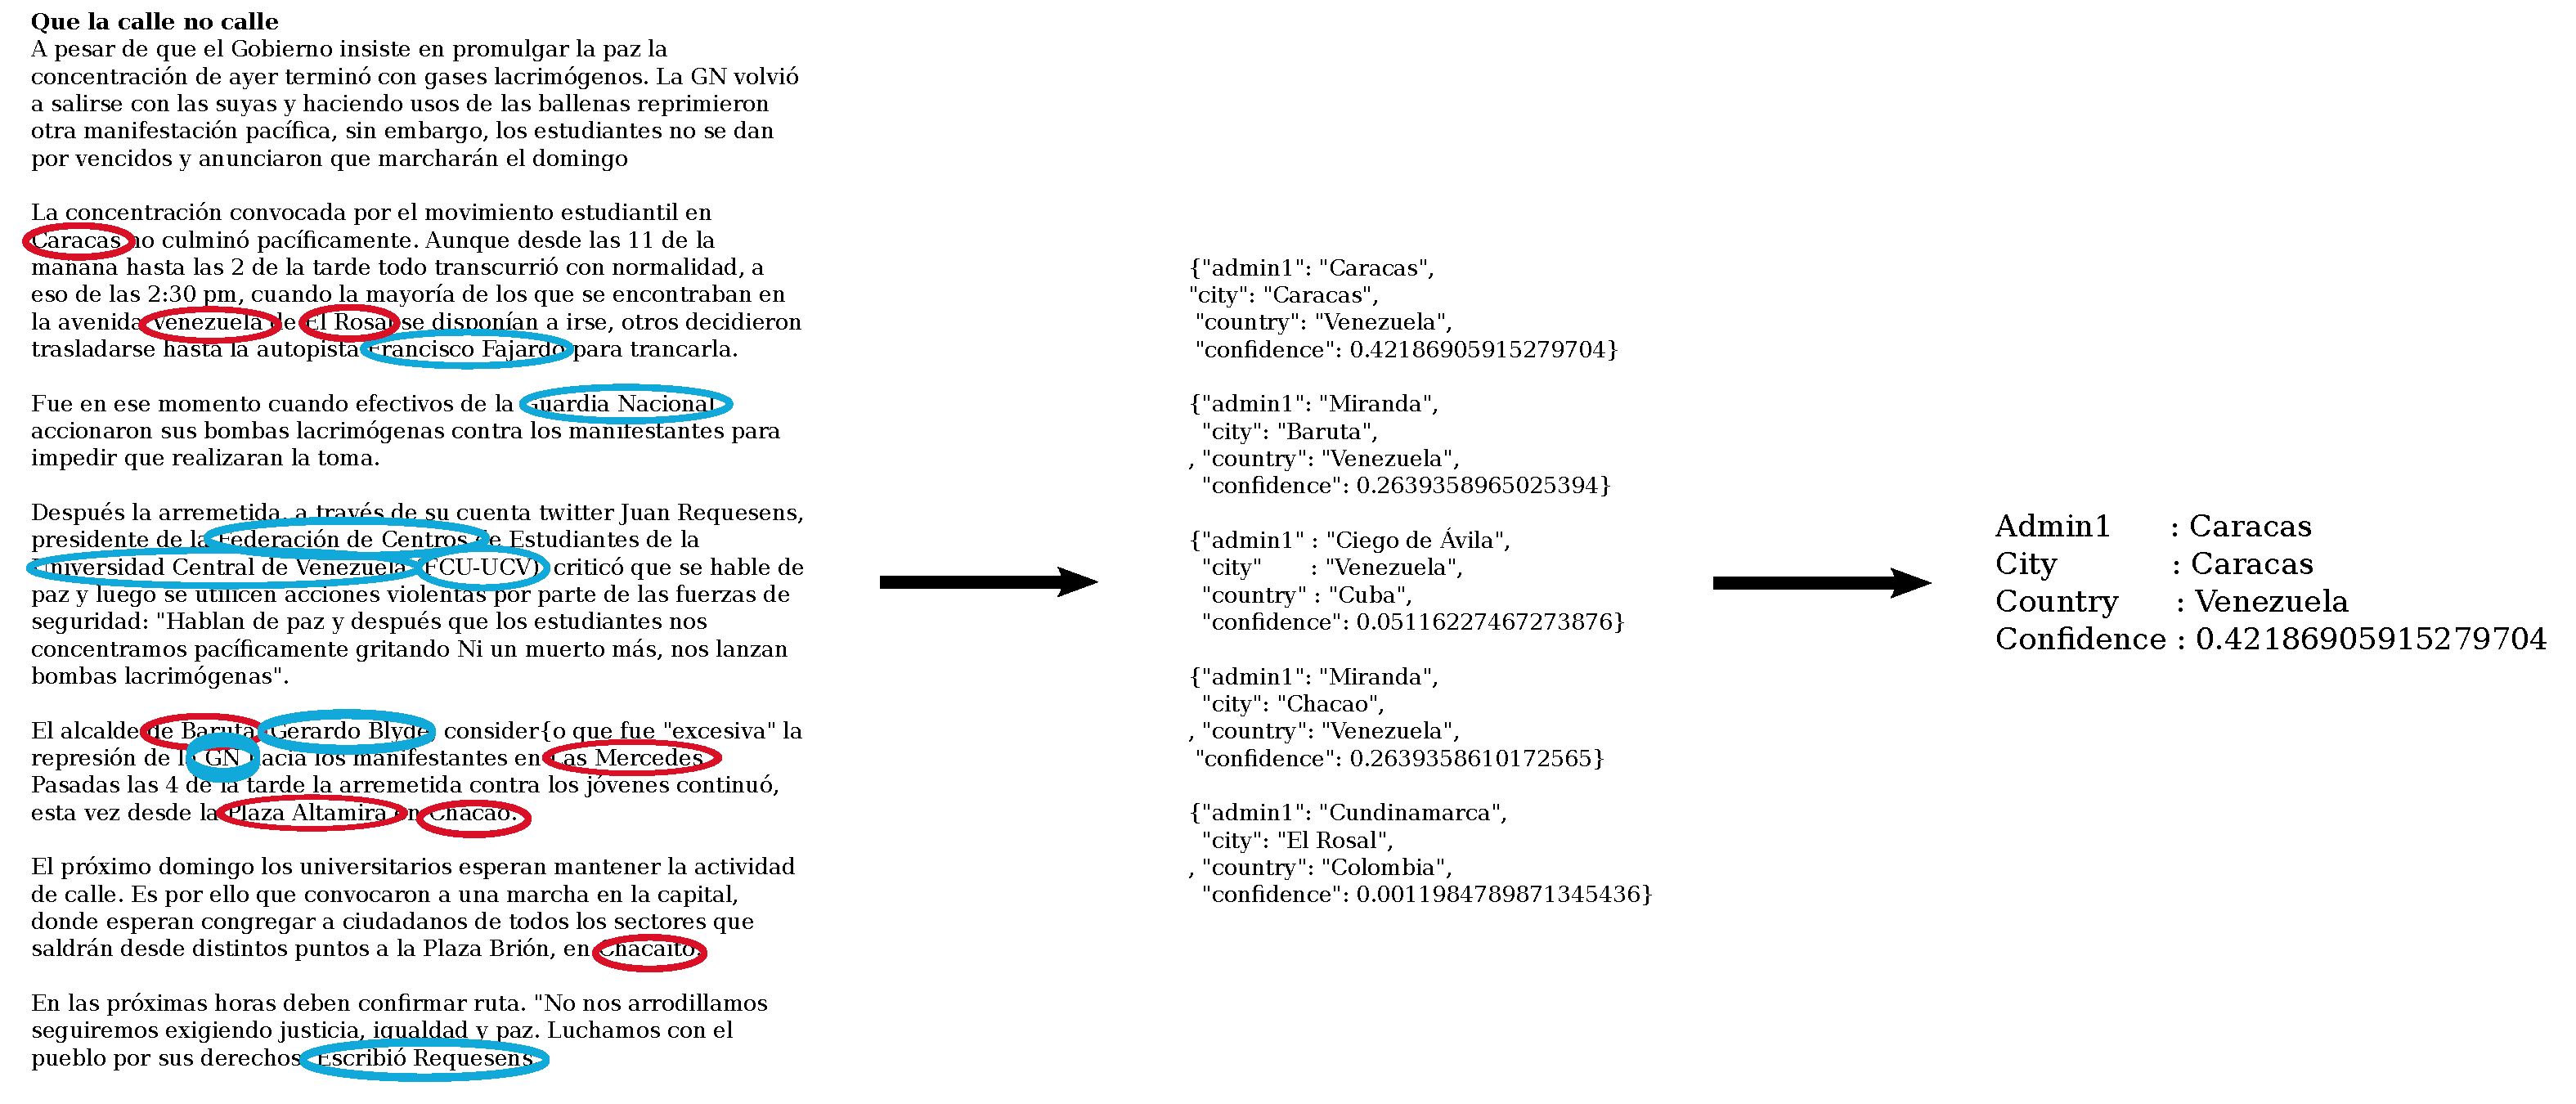
\includegraphics[width=\textwidth]{psl_pipeline2}
    \caption{Red circles denote named entities identified as locations and blue denotes other types of entities. The article talks about students planning a march on sunday.The article mentions about multiple locations like Chacao, El Roso,Francisco Fajardo highway where protests have been happening.Also, there is a reference to a quote by the mayor of Baruto.Mentions of such multiple locations makes it difficult to reason about the exact location of the protest. \sathappanc{TODO: Replace with a better protest example}}
    \label{fig:psl_example}
\end{figure*}



(GRAHAM: DO WE WANT TO SUMMARIZE SOME RESULTS HERE TOO?)

%%!TEX root = ../plannedprotest.tex

%\iffalse
%To extract the protest location from news articles, we use \emph{probabilistic soft logic} (PSL) \cite{broecheler:uai10} to build a model that performs robust, probabilistic inference given noisy signals. PSL takes a set of weighted, logic-like rules and converts them into a continuous probability distribution over the unknown truth values of logical facts. These truth values in PSL are relaxed into the $[0,1]$ interval. We use this mechanism to build a model that infers the semantic location of an article by weighing evidence coming from the Basis entity extractions and information in the World Gazatteer. 
%
%The primary rules in the model encode the effect that Basis-extracted location strings that match to gazatteer aliases are indicators of the article's location, whether they be country, state, or city aliases. Each of these implications is conjuncted with an prior for ambiguous, overloaded aliases that is proportional to the population of the gazetteer location. For example, if the string ``Los Angeles'' appears in the article, it could refer to either Los Angeles, California, or Los \'{A}ngeles in Argentina or Chile. Given no other information, our model would infer a higher truth value for the article referring to Los Angeles, California, because it has a much higher population than the other options. 
%
%The secondary rules, which are given half the weight of the primary rules, perform the same mapping of extracted strings to gazetteer aliases, but for extracted persons and organizations. Strings describing persons and organizations often include location clues (e.g., ``mayor of Buenos Aires''), but intuition suggests the correlation between the article's location and these clues may be lower than with location strings. 
%
%Finally, the model includes rules and constraints to require consistency between the different levels of geolocation, making the model place higher probability on states with its city contained in its state, which is contained in its country. As a post-processing step, we enforce this consistency explicitly by using the inferred city and its enclosing state and country, but adding these rules into the model makes the probabilistic inference prefer consistent predictions, enabling it to combine evidence at all levels.
%\fi

In this section, we briefly describe probabilistic soft logic (PSL)~\cite{kimmig2012short}, a key
component of our geocoding strategy described later.
PSL is a framework for collective probabilistic reasoning on relational domains.
PSL models have been developed in various domains, including collective classification~\cite{broecheler2010computing}, 
ontology alignment~\cite{brocheler2012probabilistic}, personalized medicine~\cite{bach2010decision}, 
opinion diffusion~\cite{bach2012scaling} , trust in social networks~\cite{huang2012probabilistic}, and graph 
summarization~\cite{memory2012graph}.
PSL represents the domain of interest as logical atoms.
It uses first order logic rules to capture the dependency structure of the domain, based on which it builds a joint probabilistic model over all atoms.
Instead of hard truth values of $0$ (false) and $1$ (true), PSL uses soft truth values relaxing the truth vlaues to the interval $[0,1]$.
The logical connectives are adapted accordingly.
This makes it easy to incorporate similarity or distance functions.

User defined \emph{predicates} are used to encode the relationships and attributes and \emph{rules} capture the  dependencies and constraints.
Each rule's antecedent is a conjunction of atoms and its consequent is a dis-junction. 
The rules can also labeled with non negative weights which are used during the inference process.
The set of predicates and weighted rules thus make up a PSL program where known truth values of ground atoms derived from observed data and unknown truth values for the remaining atoms are learned using the PSL inference.

Given a set of atoms 
$\ell = \{\ell_1,\ldots,\ell_n\}$,
an interpretation defined as 
$I : \ell \rightarrow [0,1]^n$
is a mapping from atoms to soft truth values.
PSL defines a probability distribution over all such interpretaions such that those that satisfy more ground rules are more probable.
\emph{Lukasiewicz t-norm} and its corresponding co-norm are used for defining relaxations of the logical AND and OR respectively to determine the degree to which a ground rule is satisfied.
Given an interpretation $\mathit{I}$, PSL defines the formulas for the relaxation of the logical conjunction ($\wedge$), disjunction ($\vee$), and negation ($\neg$) as follows:

\begin{align*}
\ell_1 \softand \ell_2 &= \max\{0, I(\ell_1) + I(\ell_2) - 1\},\\
\ell_1 \softor \ell_2 &= \min\{I(\ell_1) + I(\ell_2), 1\},\\
\softneg l_1 &= 1 - I(\ell_1),
\end{align*}  

The interpretation $\mathit{I}$ determines whether the rules is satisfied, if not, the \emph{distance to satisfaction}.
A rule $\mathit{r} \equiv \mathit{r_{body}} \rightarrow \mathit{r_{head}} $  is satisfied if and only if the truth value of head is at least that of the body. The rule's distance to satisfaction measures the degree to which this condition is violated.
 \newline
\begin{center} 
 $\mathit{d_r}(\mathit{I}) =$ max\{0,$\mathit{I(r_{body})} - \mathit{I(r_{head})}$\}
 \end{center}

PSL then induces a probability distribution over possible interpretations $\mathit{I}$ over the given set of ground atoms $\mathit{l} $ in the domain. 
If $\mathit{R}$ is the set of all ground rules that are instances of a rule from the system and uses only the atoms in  $\mathit{I}$ then,
the probability density function $\mathit{f}$ over $\mathit{I}$ is defined as
\begin{equation}
\label{eq:contimn1}
    f (I) = \frac{1}{Z} \text{exp}[-\sum_{r\in R} \lambda_r (d_r(I))^p]
\end{equation}
\begin{equation}
\label{eq:contimn2}
	Z = \int_{I} \text{exp} [ -\sum_{r\in R} \lambda_r (d_r(I))^p ]
\end{equation}
where~$\lambda_r$ is the weight of the rule~$r$, $Z$ is the continuous version of the normalization constant used in discrete Markov random fields, and ~$p \in \{1, 2\}$ provides a choice between two different loss functions, linear and quadratic.
The values of the atoms can be further restricted by providing linear equality and inequality constraints allowing one to encode functional constraints from the domain. 

PSL provides for two kinds of inferences:
(a) most probable explanation and (b) calculation of the marginal distributions. 
In the MPE inference given a partial interpretation with grounded atoms based on observed evidence, the PSL program infers the truth values for the unobserved atoms satisfying the most likely interpretation. 
In the second setting, given ground truth data for all atoms we can learn the weights for the rules in our PSL program.


\iffalse Most news articles and blog posts mention multiple locations, e.g.,
the location of reporting, the location of the incident, and locations corresponding
to the hometown of the newspaper. We developed a probabilistic reasoning
engine using probabilistic soft logic (PSL)
to infer the most likely city, state and country which is the main geographic focus the article.The PSL geocoder combines various types of evidence, such as named entities
such as locations, persons, and organizations identified by RLP, as
well as common names and aliases and populations of known
locations. These diverse types of evidence are used in weighted rules
that prioritize their influence on the PSL model's location
prediction. For example, extracted location tokens are strong
indicators of the content location of an article, while organization
and person names containing location names are weaker but still
informative signals; the rules corresponding to these evidence types
are weighted accordingly.

The methodology is similar to {\em Web-a-where: Geo-Tagging Web Content}.
\fi 

\begin{figure}
    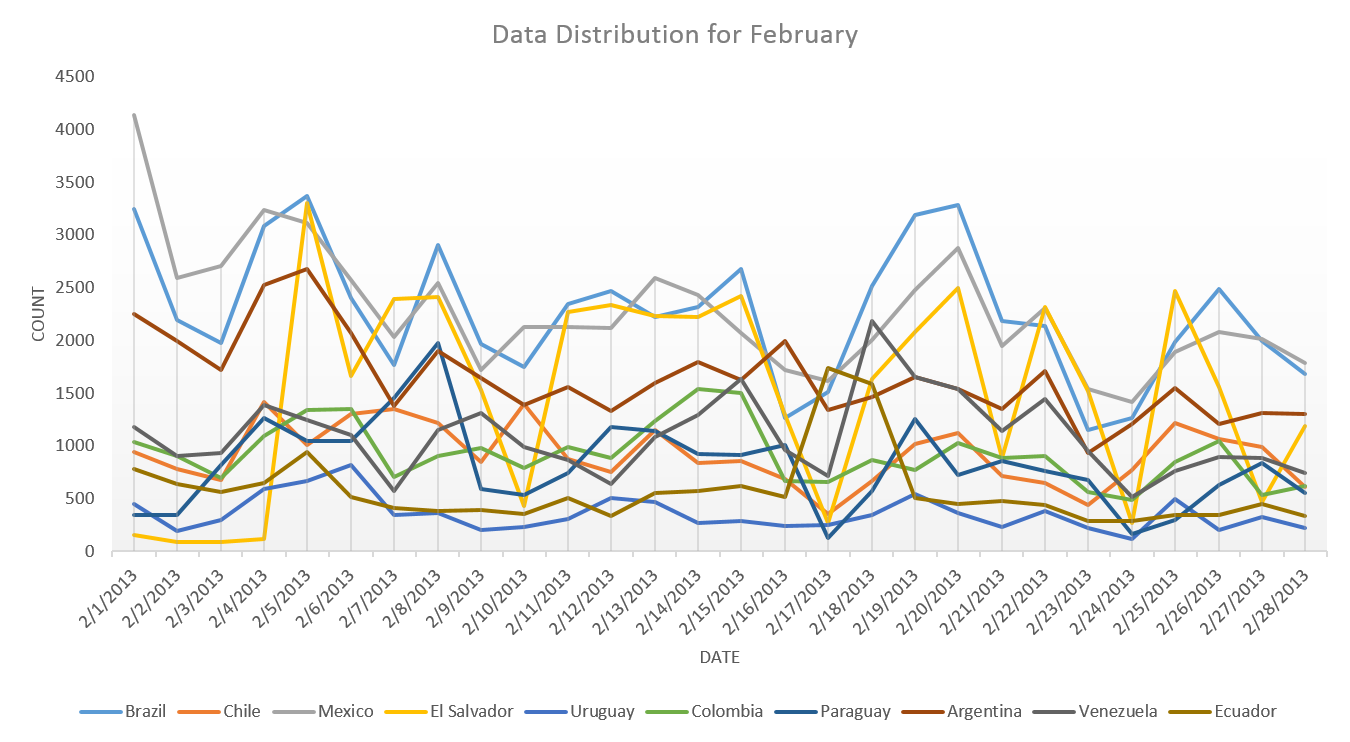
\includegraphics[width=0.5\textwidth]{rssdistribution}
    \caption{Rate of Arrival of News/Blogs}
    \label{fig:rssdistribution}
\end{figure}

